\newpage
\section{Unit Test}

Unittests werden benötigt, um die Software auf ihre Korrektheit zu überprüfen. Für diese Software werden nur Teilbereiche getestet, da viele Funktionen von der Peripherie abhängig ist.

\subsection{Quadratische Gleichung}
Für die Positionsbestimmung muss eine quadratisch Gleichung gelöst werden. Die Parameter für diese Funktion sind \si{p} und \si{q}. Diese entsprechen der Variablen aus der folgenden Gleichung:

\begin{equation}
\label{eq:unit_test_pq_formel}
x^{2} + p \cdot x + q = 0
\end{equation}

Es folgt eine Tabelle mit den Eingaben der Funktion und den dazugehörigen Ausgaben/ Rückgabewerten. 

\begin{table}[H]
\centering
\caption{Eingaben und Ausgaben der pq-Funktion}
\label{table:pq_funktion}
\begin{tabular}{|c|c|c|c|}
\hline
\multicolumn{2}{|c|}{\textbf{Eingaben}} & \multicolumn{2}{c|}{\textbf{Ergebnis}} \\ \hline
\textbf{p}         & \textbf{q}         & \textbf{x1}        & \textbf{x2}       \\ \hline
3                  & 2                  & -1                 & -2                \\ \hline
4                  & 1                  & -0,26                   & -3,73                  \\ \hline
-3                 & -9                 & 4,85                   & -1,85                  \\ \hline
\end{tabular}
\end{table}

Aus der Tabelle \ref{table:pq_funktion} wird deutlich das die Funktion korrekte Rückgabewerte liefert. Bei einer fehlerhaften Eingabe gibt die Funktion ein \si{NaN} (Not a Number) zurück.


\subsection{Abstand zweier Punkte}
Bei der Positionsbestimmung kann es dazu kommen, dass die drei Kreise sich nicht treffen. Dann haben wir zwei Bereiche indem sich der Knoten befindet. Um den korrekten Bereich zu bestimmen, wird die Funktion $determine\_point\_radius()$ benötigt. Liefert diese Funktion ein falsches Ergebnis, führt das dazu, dass die Positionsbestimmung nicht mehr korrekt ist. Der korrekte Bereich kann bestimmt werden, indem von zwei Punkten die Distanz zu einem Kreismittelpunkt bestimmt wird. Ein Punkt liegt innerhalb des Radius und der andere außerhalb. Der Punkt mit der geringsten Distanz ist der korrekte Punkt und makiert einen Eckpunkt des Bereichs indem sich der Knoten befindet. Abbildung \ref{img:figure_abstand_zweier_punkte} verdeutlicht das Problem.

\begin{figure}[H]
	\hspace*{-2.0cm}
    \subfigure[Positionsbestimmung ohne Schwankung]
    {
    	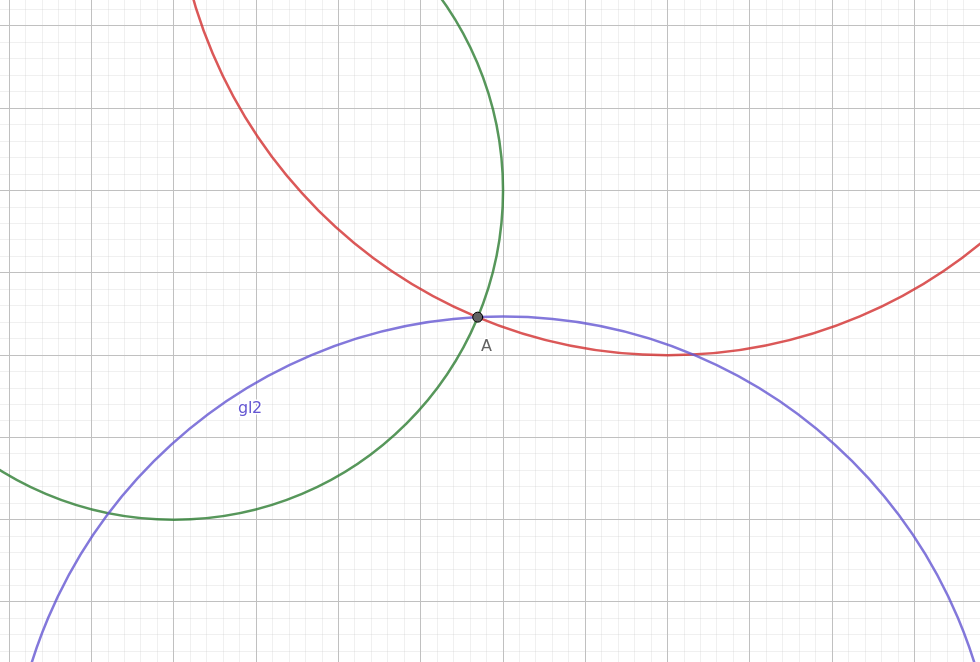
\includegraphics[width=0.6\textwidth]{images/picture_unit_test_calc_position_1.png}
    }
    \subfigure[Positionsbestimmung mit Schwankung]
    {
    	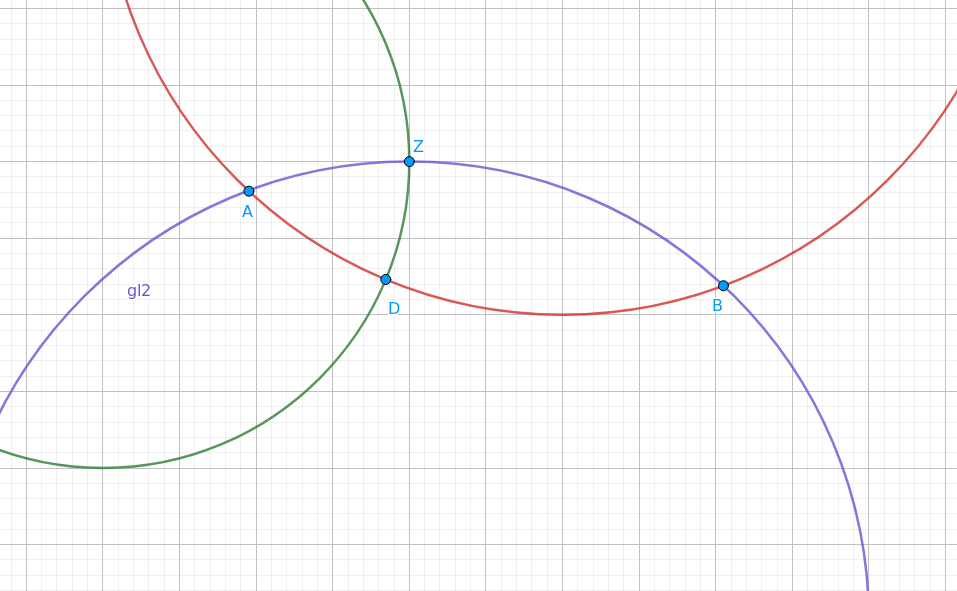
\includegraphics[width=0.6\textwidth]{images/picture_unit_test_calc_position_2.png}
    }
	\caption{Zwei Möglichkeiten der Positiosbestimmung}
	\label{img:figure_abstand_zweier_punkte}
\end{figure}

In der Abbildung \ref{img:figure_abstand_zweier_punkte} ist erkennbar, dass es durch die Schwankung zwei Bereiche geben kann. Ein Bereich durch die Eckpunkte \si{A}, \si{Z} und \si{D} und ein zweiter durch \si{B}, \si{Z} und \si{D} abgesteckt. Um nun zu bestimmen ob Punkt \si{A} oder \si{B} den Bereich ausgegangen von dem grünen Kreis kennzeichnet wird der Abstand zum Kreismittelpunkt vom grünen Kreis berechnet. Die Funktion wird mit den folgenden zwei Punkten und der Kreisgleichung getestet.

\begin{equation*}
\label{eq:unit_test_abstand_zweier_punkte}
\begin{split}
P_{A}: \; (3,9528 \;|\; 2,8069)\\
P_{B}: \; (7,0504 \;|\; 2,1899)\\
(x - 3)^{2} + (y - 3)^{2} = 2^{2}
\end{split}
\end{equation*}

Punkt \si{A} ist der korrekte Punkt, weil sein Abstand zum Kreismittelpunkt kleiner ist als von Punkt \si{B} ($0.9721 < 4.1306$) und daher sollte er von der Funktion zurückgegeben werden. Die Funktion funktioniert wie erwartet fehlerfrei.

\subsection{Positionsbestimmung}
Zur Bestimmung der Position braucht die Funktion $calc_position()$ drei Parameter. Diese sind die drei Kreise die sich im einem Schnittpunkt schneiden oder ein Bereich aufspannen. Für den Fall das alle drei Kreise einen gemeinsamen Schnittpunkt haben gibt die Funktion dreimal die X/Y-Koordinaten zurück. Bei einem Bereich werden die X/Y-Koordinaten der Eckpunkte zurückgegeben. Die Funktion wird mit den folgenden Kreisgleichungen getestet.  Zuerst ein test wobei es ein gemeinsamen Schnittpunkt gibt.

\begin{equation*}
\label{eq:unit_test_positionsbestimmung}
\begin{split}
(x - 3)^{2} + (y - 3)^{2} = 2^{2} \\
(x - 6)^{2} + (y - 2)^{2} = 2^{2} \\
(x - 4)^{2} + (y - 1,8693)^{2} = 2^{2}
\end{split}
\end{equation*}
Der Schnittpunkt der drei Kreise ist $( 4,8872 \;|\; 3,6618)$. Dies gibt auch die Funktion zurück. Als nächtes wird der Rückgabewert bei keinem gemeinsamen Schittpunkt untersucht.

\begin{equation*}
\label{eq:unit_test_positionsbestimmung}
\begin{split}
(x - 3)^{2} + (y - 3)^{2} = 2^{2} \\
(x - 6)^{2} + (y - 2)^{2} = 2^{2} \\
(x - 4)^{2} + (y - 5)^{2} = 2^{2}
\end{split}
\end{equation*}

Die obigen drei Kreise haben keinen gemeinsamen Schittpunkt. Die Funktion gibt die folgenden Koordinaten der Eckpunkte zurück.

\begin{equation*}
\label{eq:unit_test_positionsbestimmung_2}
\begin{split}
P_{A}: \; (4,8872 \;|\; 3,6618)\\
P_{B}: \; (4,9832 \;|\; 3,2583)\\
P_{C}: \; (4,2794 \;|\; 3,0196)
\end{split}
\end{equation*}

In beiden Fällen ist der Rückgabewert der Funktion korrekt. Somit funktioniert die Funktion wie erwartet.






